%%
%% This is file `sample-sigconf.tex',
%% generated with the docstrip utility.
%%
%% The original source files were:
%%
%% samples.dtx  (with options: `sigconf')
%%
%% IMPORTANT NOTICE:
%%
%% For the copyright see the source file.
%%
%% Any modified versions of this file must be renamed
%% with new filenames distinct from sample-sigconf.tex.
%%
%% For distribution of the original source see the terms
%% for copying and modification in the file samples.dtx.
%%
%% This generated file may be distributed as long as the
%% original source files, as listed above, are part of the
%% same distribution. (The sources need not necessarily be
%% in the same archive or directory.)
%%
%% The first command in your LaTeX source must be the \documentclass command.
\documentclass[sigplan,screen,10pt,anonymous,review]{acmart}

\providecommand{\tightlist}{%
  \setlength{\itemsep}{0pt}\setlength{\parskip}{0pt}}

%%
%% \BibTeX command to typeset BibTeX logo in the docs
\AtBeginDocument{%
  \providecommand\BibTeX{{%
    \normalfont B\kern-0.5em{\scshape i\kern-0.25em b}\kern-0.8em\TeX}}}

%% Rights management information.  This information is sent to you
%% when you complete the rights form.  These commands have SAMPLE
%% values in them; it is your responsibility as an author to replace
%% the commands and values with those provided to you when you
%% complete the rights form.

%%
%% Submission ID.
%% Use this when submitting an article to a sponsored event. You'll
%% receive a unique submission ID from the organizers
%% of the event, and this ID should be used as the parameter to this command.
%%\acmSubmissionID{123-A56-BU3}

%%
%% The majority of ACM publications use numbered citations and
%% references.  The command \citestyle{authoryear} switches to the
%% "author year" style.
%%
%% If you are preparing content for an event
%% sponsored by ACM SIGGRAPH, you must use the "author year" style of
%% citations and references.
%% Uncommenting
%% the next command will enable that style.
%%\citestyle{acmauthoryear}
%%
%% end of the preamble, start of the body of the document source.

\usepackage{listings}

\usepackage{color}
\usepackage{fancyvrb}
\newcommand{\VerbBar}{|}
\newcommand{\VERB}{\Verb[commandchars=\\\{\}]}
\DefineVerbatimEnvironment{Highlighting}{Verbatim}{commandchars=\\\{\}}
% Add ',fontsize=\small' for more characters per line
\newenvironment{Shaded}{}{}
\newcommand{\AlertTok}[1]{\textcolor[rgb]{1.00,0.00,0.00}{\textbf{#1}}}
\newcommand{\AnnotationTok}[1]{\textcolor[rgb]{0.38,0.63,0.69}{\textbf{\textit{#1}}}}
\newcommand{\AttributeTok}[1]{\textcolor[rgb]{0.49,0.56,0.16}{#1}}
\newcommand{\BaseNTok}[1]{\textcolor[rgb]{0.25,0.63,0.44}{#1}}
\newcommand{\BuiltInTok}[1]{#1}
\newcommand{\CharTok}[1]{\textcolor[rgb]{0.25,0.44,0.63}{#1}}
\newcommand{\CommentTok}[1]{\textcolor[rgb]{0.38,0.63,0.69}{\textit{#1}}}
\newcommand{\CommentVarTok}[1]{\textcolor[rgb]{0.38,0.63,0.69}{\textbf{\textit{#1}}}}
\newcommand{\ConstantTok}[1]{\textcolor[rgb]{0.53,0.00,0.00}{#1}}
\newcommand{\ControlFlowTok}[1]{\textcolor[rgb]{0.00,0.44,0.13}{\textbf{#1}}}
\newcommand{\DataTypeTok}[1]{\textcolor[rgb]{0.56,0.13,0.00}{#1}}
\newcommand{\DecValTok}[1]{\textcolor[rgb]{0.25,0.63,0.44}{#1}}
\newcommand{\DocumentationTok}[1]{\textcolor[rgb]{0.73,0.13,0.13}{\textit{#1}}}
\newcommand{\ErrorTok}[1]{\textcolor[rgb]{1.00,0.00,0.00}{\textbf{#1}}}
\newcommand{\ExtensionTok}[1]{#1}
\newcommand{\FloatTok}[1]{\textcolor[rgb]{0.25,0.63,0.44}{#1}}
\newcommand{\FunctionTok}[1]{\textcolor[rgb]{0.02,0.16,0.49}{#1}}
\newcommand{\ImportTok}[1]{#1}
\newcommand{\InformationTok}[1]{\textcolor[rgb]{0.38,0.63,0.69}{\textbf{\textit{#1}}}}
\newcommand{\KeywordTok}[1]{\textcolor[rgb]{0.00,0.44,0.13}{\textbf{#1}}}
\newcommand{\NormalTok}[1]{#1}
\newcommand{\OperatorTok}[1]{\textcolor[rgb]{0.40,0.40,0.40}{#1}}
\newcommand{\OtherTok}[1]{\textcolor[rgb]{0.00,0.44,0.13}{#1}}
\newcommand{\PreprocessorTok}[1]{\textcolor[rgb]{0.74,0.48,0.00}{#1}}
\newcommand{\RegionMarkerTok}[1]{#1}
\newcommand{\SpecialCharTok}[1]{\textcolor[rgb]{0.25,0.44,0.63}{#1}}
\newcommand{\SpecialStringTok}[1]{\textcolor[rgb]{0.73,0.40,0.53}{#1}}
\newcommand{\StringTok}[1]{\textcolor[rgb]{0.25,0.44,0.63}{#1}}
\newcommand{\VariableTok}[1]{\textcolor[rgb]{0.10,0.09,0.49}{#1}}
\newcommand{\VerbatimStringTok}[1]{\textcolor[rgb]{0.25,0.44,0.63}{#1}}
\newcommand{\WarningTok}[1]{\textcolor[rgb]{0.38,0.63,0.69}{\textbf{\textit{#1}}}}


\begin{document}

%%
%% The "title" command has an optional parameter,
%% allowing the author to define a "short title" to be used in page headers.
\title{End-User Software Customization by Direct Manipulation of Tabular
Data}

%%
%% The "author" command and its associated commands are used to define
%% the authors and their affiliations.
%% Of note is the shared affiliation of the first two authors, and the
%% "authornote" and "authornotemark" commands
%% used to denote shared contribution to the research.

\author{Geoffrey Litt}
\affiliation{%
  \institution{Massachusetts Institute of Technology}
  \city{Cambridge, MA}
  \country{USA}
}
\email{glitt@mit.edu}

\author{Daniel Jackson}
\affiliation{%
  \institution{Massachusetts Institute of Technology}
  \city{Cambridge, MA}
  \country{USA}
}
\email{dnj@csail.mit.edu}

\author{Tyler Millis}
\affiliation{%
  \institution{Massachusetts Institute of Technology}
  \city{Cambridge, MA}
  \country{USA}
}
\email{tmillis@mit.edu}

\author{Jessica Quaye}
\affiliation{%
  \institution{Massachusetts Institute of Technology}
  \city{Cambridge, MA}
  \country{USA}
}
\email{jquaye@mit.edu}

%%
%% By default, the full list of authors will be used in the page
%% headers. Often, this list is too long, and will overlap
%% other information printed in the page headers. This command allows
%% the author to define a more concise list
%% of authors' names for this purpose.
% \renewcommand{\shortauthors}{Trovato and Tobin, et al.}

%%
%% The abstract is a short summary of the work to be presented in the
%% article.
\begin{abstract}
  In this paper we introduce \emph{data-driven customization}, a new way
  for end users to extend software by direct manipulation without doing
  traditional programming. We augment existing user interfaces with a
  table view showing the structured data inside the application. When
  users edit the table, their changes are reflected in the original UI.
  This simple model accommodates a spreadsheet formula language and
  custom data editing widgets, providing enough power to implement a
  variety of useful extensions.

  We illustrate the approach with Wildcard, a browser extension that
  implements data-driven customization for existing applications using
  web scraping. Through concrete examples, we show that this paradigm
  can support extensions to many real websites, ranging from sorting and
  filtering existing data to adding entire new features. We share
  reflections from our experiences using Wildcard, on both its strengths
  and limitations relative to other customization approaches. Finally,
  we explore how this paradigm might lead to new software architectures
  that encourage this form of end-user customization.
\end{abstract}

%%
%% The code below is generated by the tool at http://dl.acm.org/ccs.cfm.
%% Please copy and paste the code instead of the example below.
%%
%% From HERE
\begin{CCSXML}
<ccs2012>
<concept>
<concept_id>10011007.10011006.10011066.10011069</concept_id>
<concept_desc>Software and its engineering~Integrated and visual development environments</concept_desc>
<concept_significance>500</concept_significance>
</concept>
</ccs2012>
\end{CCSXML}

\ccsdesc[500]{Software and its engineering~Integrated and visual development environments}
% To HERE

%%
%% Keywords. The author(s) should pick words that accurately describe
%% the work being presented. Separate the keywords with commas.
\keywords{end-user programming, software customization, web browser extensions}

%% A "teaser" image appears between the author and affiliation
%% information and the body of the document, and typically spans the
%% page.
%\begin{teaserfigure}
%  \includegraphics[width=\textwidth]{sampleteaser}
%  \caption{Seattle Mariners at Spring Training, 2010.}
%  \Description{Enjoying the baseball game from the third-base
%  seats. Ichiro Suzuki preparing to bat.}
%  \label{fig:teaser}
%\end{teaserfigure}

%%
%% This command processes the author and affiliation and title
%% information and builds the first part of the formatted document.
\maketitle

\hypertarget{introduction}{%
\section{Introduction}\label{introduction}}

Many applications don't meet the precise needs of their users, and it is
impossible for developers to anticipate everyone's unique requirements.
End user customization systems can help close this gap, by empowering
non-programmers to modify their software to satisfy their personal
goals.

Many end user customization systems
\citep{cook2007, bolin2005, leshed2008, chasins2018} offer a scripting
model. They use various strategies to make programming more
approachable: friendly syntax, a visual programming environment, or
macro recording to bootstrap from concrete demonstrations. But all these
techniques build on the same fundamental foundation: an imperative
programming model, with statements, mutable variables, and loops.

We have known for decades about an alternative: \emph{direct
manipulation} \citep{shneiderman1983}, where ``visibility of the object
of interest'' replaces ``complex command language syntax.'' Direct
manipulation is the \emph{de facto} standard in GUIs today, but when it
comes to customizing those GUIs, it is rarely to be found. Switching
from using an application to customizing it via scripting requires an
abrupt shift in interaction model, and can pose a steep learning barrier
for users not familiar with programming.

We subscribe to MacLean et al.'s vision of a ``gentle slope''
\citep{maclean1990} free of such ``cliffs,'' where users should only
need to make minimal and incremental investments in skill to achieve
their desired customizations. We seek to contribute to this gentle slope
with a new method for customizing software via direct manipulation,
taking inspiration from visual database query interfaces and
spreadsheets, which have successfully enabled millions of end users to
compute with data through direct manipulation.

In our proposed paradigm, \emph{data-driven customization}, an
application's UI is augmented with a table view where the user can see
and manipulate the application's internal data. These changes don't just
apply to the table; they also result in immediate changes to the
application's original user interface. The user can sort/filter data in
the UI, inject annotations, pull in related information from other web
services, and more, all using the table as a mediating interface.
Interacting with the table view resembles interacting with a familiar
spreadsheet, but results in customizing an existing application.

\begin{figure*}
\hypertarget{fig:overview}{%
\centering
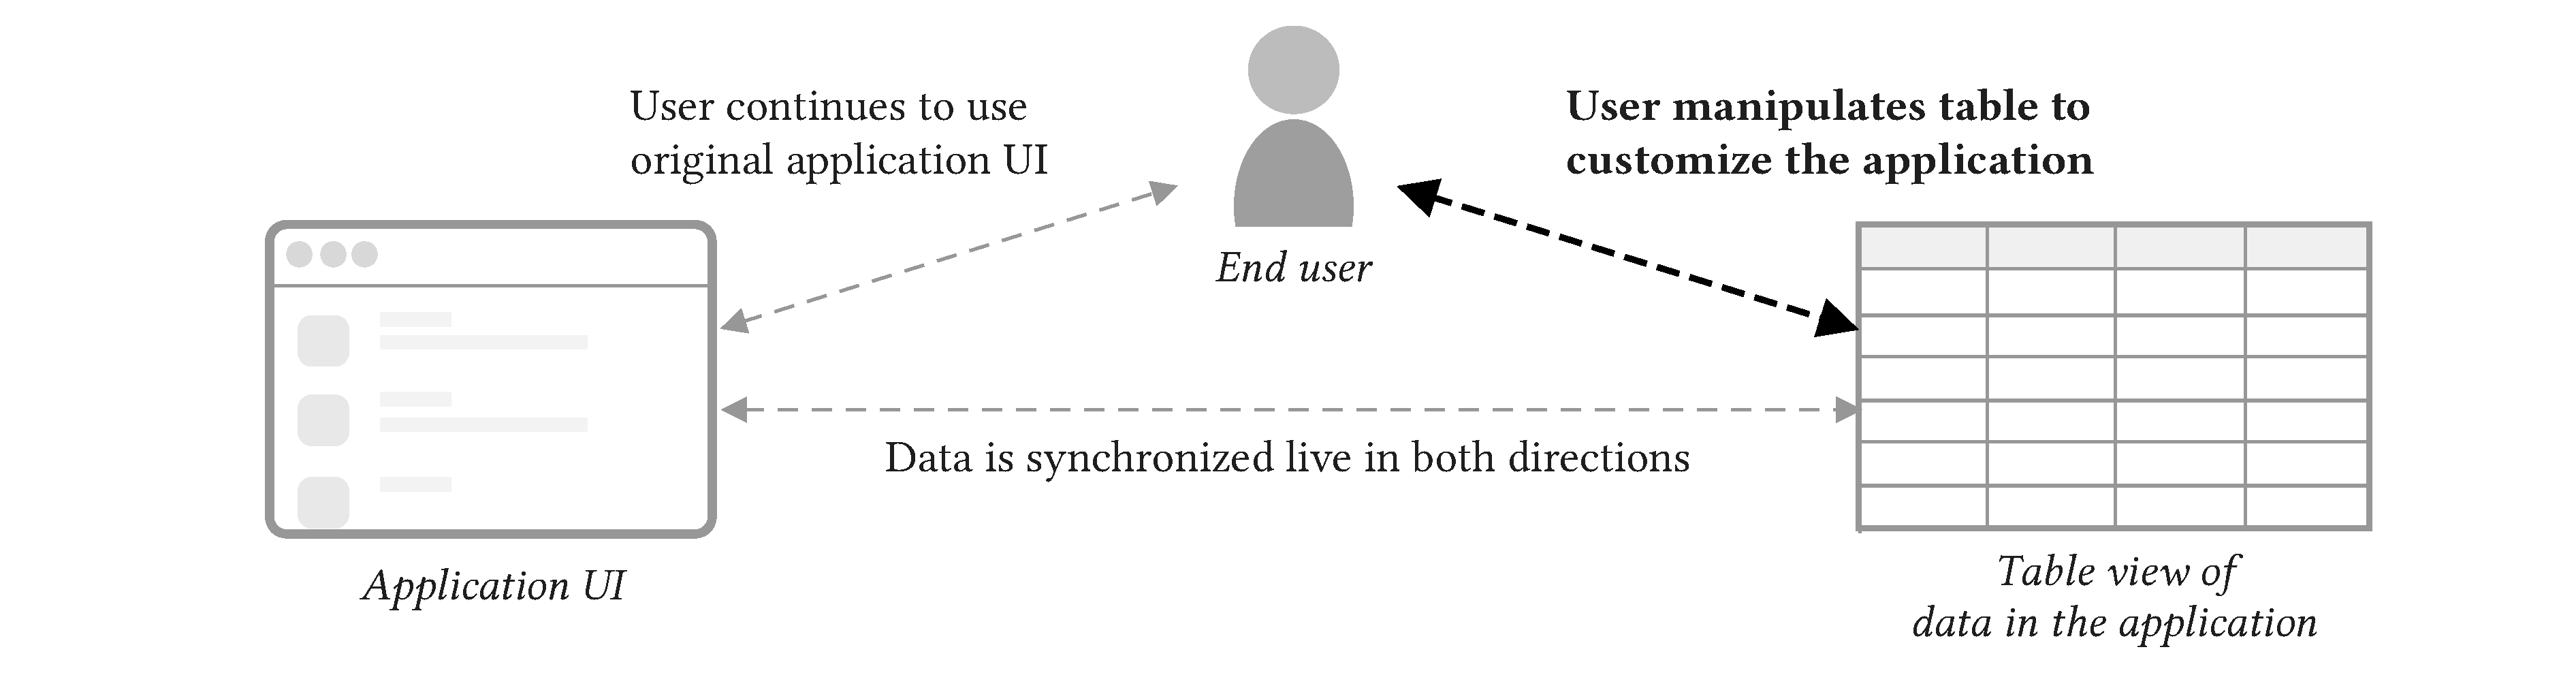
\includegraphics[width=\textwidth]{media/overview.eps}
\caption{An overview of data-driven customization}\label{fig:overview}
}
\end{figure*}

We have developed a browser extension called Wildcard which uses web
scraping techniques to implement data-driven customization for existing
Web applications. In Section~\ref{sec:example}, we concretely
demonstrate the end user experience of using Wildcard to add features to
a news website.

In Section~\ref{sec:architecture}, we explain the system architecture of
data-driven customization. We focus on the \emph{table adapter}
abstraction, which allows many different types of underlying data to be
bidirectionally mapped to a table. We describe several types of table
adapters we've built in Wildcard, and also describe future adapters
supported by the general paradigm.

We have successfully used Wildcard to build customizations for 11
different websites that serve our own personal needs. In
Section~\ref{sec:reflections}, we present reflections from this process.
We outline the kinds of customizations we were able to build,
limitations we encountered, and some of the challenges of writing
scraping logic.

In Section~\ref{sec:visions}, we discuss some key themes from our work:

\begin{itemize}
\tightlist
\item
  \emph{Customization by direct manipulation}: We discuss further how
  data-driven customization relates to a gentle slope of customization.
  We suggest that an important point on this slope is the ability to
  customize an application by directly seeing and changing its data,
  rather than by writing imperative scripts.
\item
  \emph{Semantic wrappers}: Typically, tools that don't rely on official
  extension APIs resort to offering low-level APIs for customization.
  Instead, we propose a community-maintained library of semantic
  wrappers around existing applications, enabling end users to work with
  domain data rather than low-level representations.
\end{itemize}

data-driven customization relates to existing work in many areas. Our
goals overlap with many software customization tools, and our methods
overlap with direct manipulation interfaces for working with structured
data, including visual database query systems and spreadsheets. We
explore these connections in Section~\ref{sec:related-work}.

Finally, in Section~\ref{sec:conclusion}, we conclude and describe
opportunities for future work.

\hypertarget{sec:example}{%
\section{Example Scenario}\label{sec:example}}

To concretely illustrate the user experience of data-driven
customization, we present a scenario of customizing
\href{https://news.ycombinator.com/}{Hacker News}, a popular tech news
aggregator. Figure~\ref{fig:hacker-news} shows accompanying screenshots.

\begin{figure*}
\hypertarget{fig:hacker-news}{%
\centering
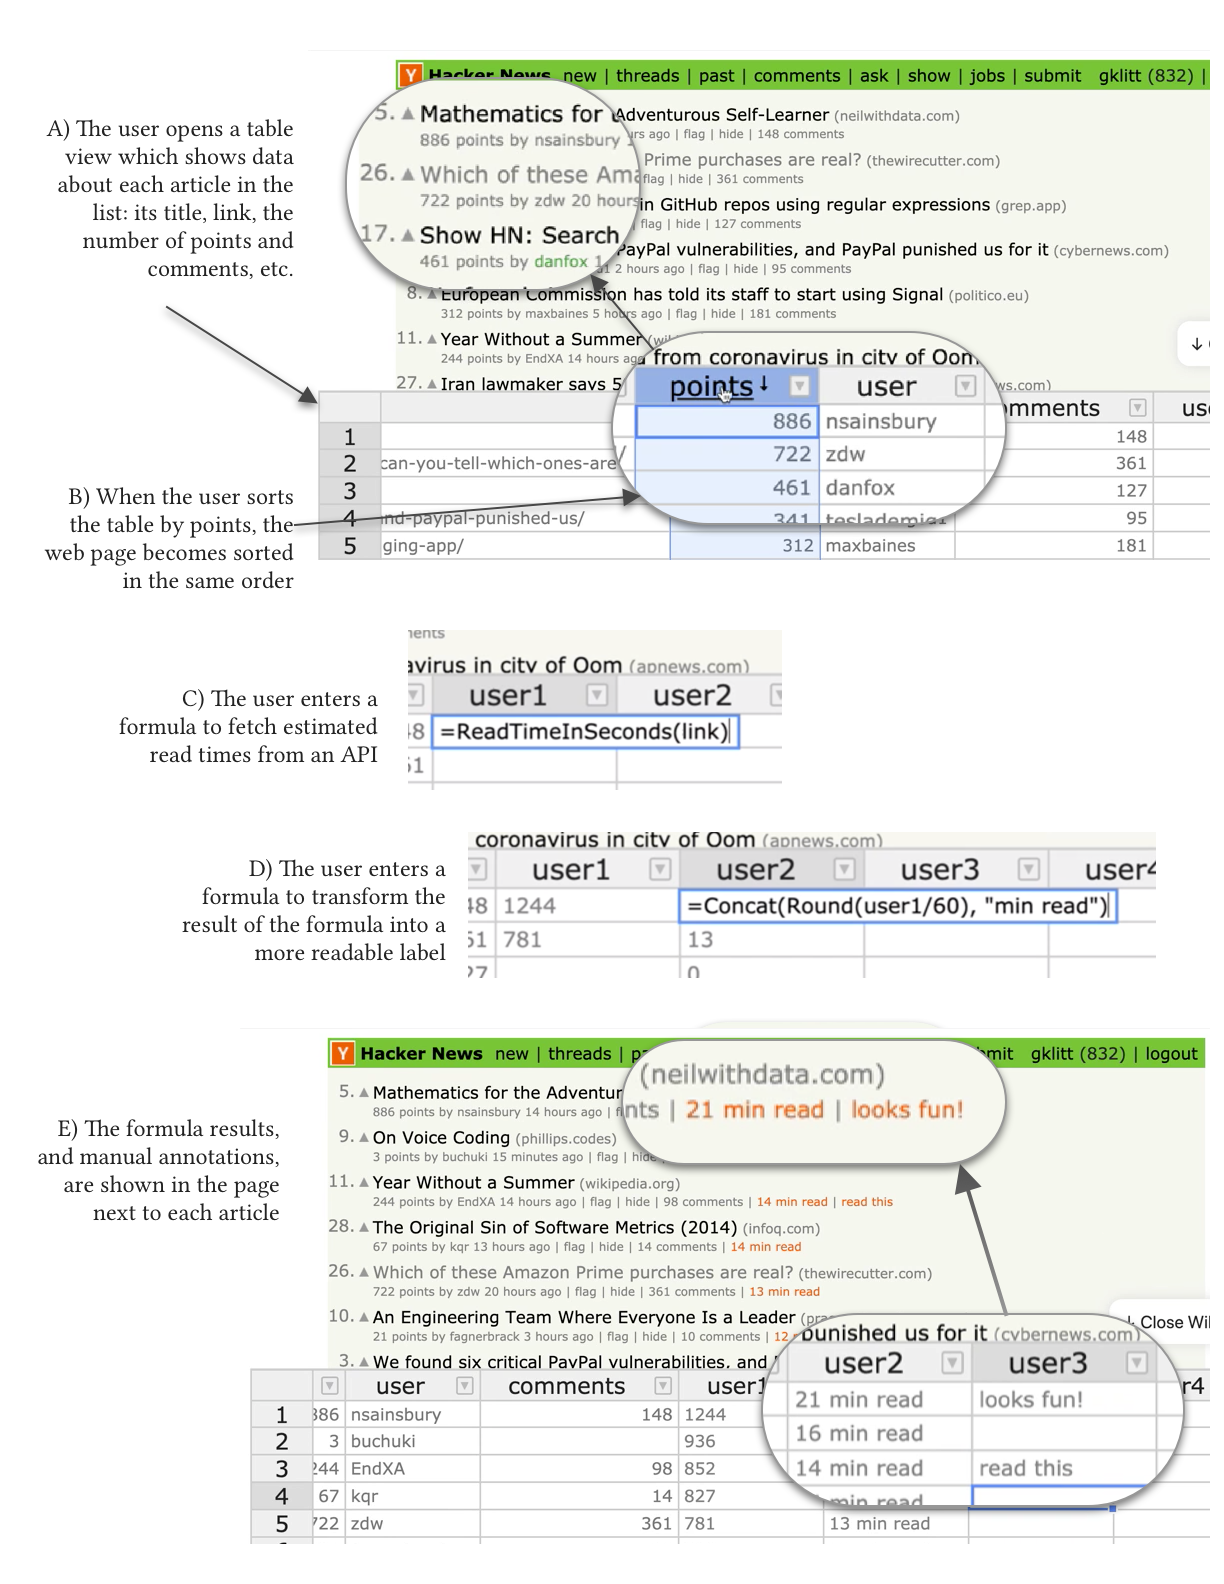
\includegraphics[width=\textwidth]{media/hacker-news.png}
\caption{Customizing Hacker News by interacting with a table view}\label{fig:hacker-news}
}
\end{figure*}

\textbf{Opening the table}: When the user opens Hacker News in a browser
equipped with the Wildcard extension, they see a table at the bottom of
the page. It contains a row for each link on the homepage, listing
information like the title, URL, submitter username, number of points,
and number of comments (Figure~\ref{fig:hacker-news}, Note A). The end
user didn't need to do any work to create this table, because a
programmer previously created an adapter to extract data from this
particular website, and contributed it to a shared library of adapters
integrated into Wildcard.

\textbf{Sorting by points}: First, the user decides to change the
ranking of links on the homepage. Hacker News itself uses a ranking
algorithm in which the position of an article depends not only on its
point count (a measure of popularity), but also on how long it has been
on the site. If the user hasn't been checking the site frequently, it's
easy to miss a popular article that has fallen lower on the list.
Sorting the page just by points would achieve a more stable ranking.

To achieve this ordering, the user simply clicks on the ``points''
column header in the table. This sorts the table view by points, and the
website UI also becomes sorted in the same order
(Figure~\ref{fig:hacker-news}, Note B). Internally, Wildcard has changed
the website's DOM to synchronize it with the sort order of the table.
This sort predicate is also persisted in the browser and reapplied
automatically the next time the user loads the page, so they can always
browse the page sorted by points.

\textbf{Adding estimated read times}: Next, the user decides to attempt
a more substantial customization: adding estimated read times to each
article, in order to prioritize reading deeper content.

The table contains additional empty columns where the user can enter
spreadsheet-like formulas to compute derived values. The user enters a
formula into the first column, which is named \texttt{user1} by default
(Figure~\ref{fig:hacker-news}, Note C):

\begin{verbatim}
=ReadTimeInSeconds(link)
\end{verbatim}

This formula calls a built-in function \texttt{ReadTimeInSeconds} that
uses a third-party public web API to compute an estimated read time for
the URL's contents. The \texttt{link} argument in the formula refers to
a column name in the table; the formula is automatically evaluated
across all rows in the table, using the value of \texttt{link} for each
row.

The user clicks the \texttt{user1} column header to sort the articles on
the page in descending order of estimated read time. They would also
like to display the read times in the page, but a number in seconds
isn't the most legible format, so they enter another formula in the
\texttt{user2} column:

\begin{verbatim}
=Concat(Round(user1/60), "min read")
\end{verbatim}

This formula converts seconds to minutes by dividing by 60 and rounding
to the nearest integer, and concatenates the result with a string label,
producing results like ``21 min read''.

Finally, the user clicks a menu option in the table header to display
the contents of this new column in the original page
(Figure~\ref{fig:hacker-news}, Note D). Each article on the page now
shows an annotation with the estimated read time in minutes. (The
formatting of annotations was determined by the programmer who created
the adapter for Hacker News.)

\textbf{Adding manual annotations}: The user can also manually add notes
to the table, by simply entering values into the table without using
formulas. In this case, the user jots down a few notes in another column
about articles they might want to read, and the notes appear in the page
next to the read times (Figure~\ref{fig:hacker-news}, Note D). The
annotations are also stored in the browser's local storage so they can
be retrieved on future visits.

\textbf{Filtering out visited links}: Another way to use formulas to
customize Hacker News is to filter out articles the user has already
read. (We omit this example from the figure for brevity.) The user can
call a built-in function that returns a boolean depending on whether a
URL is in the browser's history:

\begin{verbatim}
=Visited(link)
\end{verbatim}

They can then filter the table to only contain rows where this formula
column contains \texttt{false}; links that the user has already visited
are hidden both from the table view and the original page. This is an
example of a customization that the original website could not have
implemented, since websites don't have access to the browser history for
privacy reasons. But by using Wildcard, the user was able to implement
the customization locally, without needing to expose their browser
history to Hacker News.

This scenario has shown a few examples of how data-driven customizations
can help a user improve their experience of a website.
Section~\ref{sec:reflections} explains many other use cases and contexts
where the technique applies, but first we explain how the system works
internally.

\hypertarget{sec:architecture}{%
\section{System architecture}\label{sec:architecture}}

\begin{figure}
\hypertarget{fig:table-adapter}{%
\centering
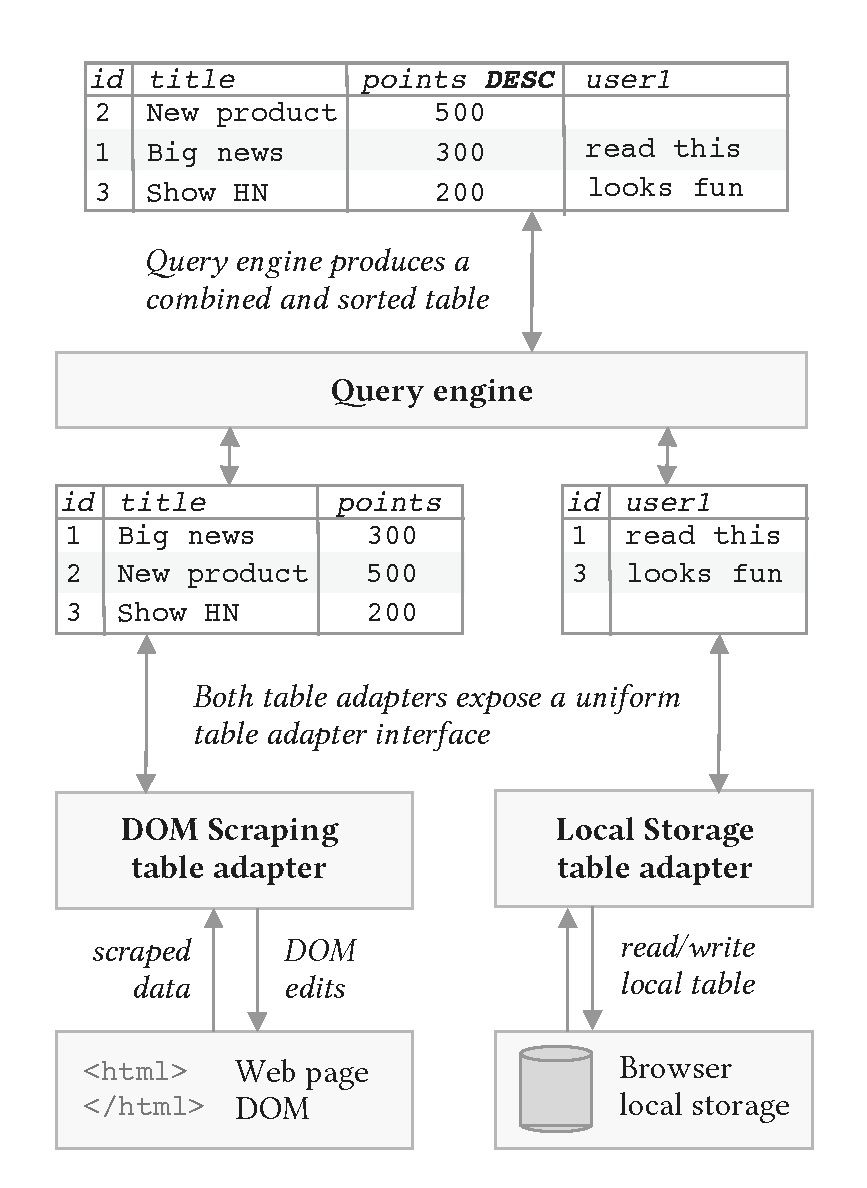
\includegraphics[width=\columnwidth]{media/table-adapter.eps}
\caption{The table adapter architecture}\label{fig:table-adapter}
}
\end{figure}

Figure~\ref{fig:table-adapter} summarizes the overall architecture of
data-driven customization, using a simplified illustration of the Hacker
News example scenario. The name and points value for each article is
scraped from the web page DOM, and user annotations are loaded from the
brower's local storage.

First, the web page and the browser storage are each wrapped by a
\textbf{table adapter}, which defines a bidirectional mapping between an
underlying data source and a table.

In addition to a \emph{read mapping} for how the underlying data should
be represented as a table, it also has a \emph{write mapping} defining
the effects that edits have on the original data source. The local
storage adapter has a trivial mapping: it loads a table of data stored
in the browser, and persists edits to that state. The mapping logic of
the DOM scraping adapter is much more involved. It implements web
scraping logic to produce a table of data from the web page, and turns
edits into DOM manipulations, such as reordering rows of data on the
page.

The two tables are then combined into a single table for the user to
view and edit. The \textbf{query engine} is responsible for creating
this combined view, and routing the user's edits back to the individual
table adapters. In this example, the query engine has joined the two
tables together by a shared ID column, and sorted the result by the
points column.

We now examine each component of the system in more detail.

\hypertarget{table-adapters}{%
\subsection{Table adapters}\label{table-adapters}}

A key idea in data-driven customization is that a wide variety of data
sources can be mapped to a generic table abstraction. In a relational
database, the table matches the underlying storage format, but in
data-driven customization, the table is merely an \emph{interface
layer}. The data shown in the table is a projection of some underlying
state, and edits to the table can have complex effects on the underlying
state.

Here we describe the three types of table adapters we have built so far
in Wildcard. These do not represent an exhaustive set of all possible
table adapters---in Section~\ref{sec:visions} we discuss other types of
adapters that would fit well into the general paradigm.

\hypertarget{dom-scraping-adapters}{%
\subsubsection{DOM scraping adapters}\label{dom-scraping-adapters}}

DOM scraping adapters enable Wildcard to interface with an existing
website UI. A DOM scraping adapter fulfills the standard web scraping
task of extracting a table of data from the DOM, but it must also handle
the reverse direction: manipulating the DOM to reflect edits to the
table.

Currently, we require DOM scraping adapters to be programmed manually
for each website using Javascript code. It might seem that this
prohibits non-programmer users from using the system, but we solve this
problem via a shared repository of adapters. Once an adapter is
programmed for a website, it is added to a shared code repository,
enabling any end user to perform customizations on that website.

There are other ways a DOM scraping adapter could be produced which
would reduce this dependence on programmers: an end user could specify
the scraping logic via demonstration, or the desired data table could be
automatically inferred from the page. While we are interested in these
techniques and discuss them later in Section~\ref{sec:visions}, we
believe that a shared repository of manually programmed adapters is a
pragmatic starting point; given that many users visit the same popular
websites,a critical mass of adapters could serve the needs of many
users.

To ease the burden on programmers of creating these adapters, we have
created a framework makes the process feel more like writing
unidirectional scraping code than performing a complex bidirectional
synchronization. The key idea is this: programmers return pointers to
DOM elements representing table rows and table cells; Wildcard extracts
data from these DOM elements, but it also uses the pointers to
synchronize table edits back into the page. For example, when the user
sorts the table, the DOM elements representing the table rows are moved
around in the DOM to reflect the new sorted order.

\begin{figure*}

\begin{Shaded}
\begin{Highlighting}[]
\KeywordTok{const}\NormalTok{ HNAdapter }\OperatorTok{=} \AttributeTok{createDomScrapingAdapter}\NormalTok{(}\OperatorTok{\{}
  \DataTypeTok{name}\OperatorTok{:} \StringTok{"Hacker News"}\OperatorTok{,}

  \CommentTok{// Specify when the adapter should be enabled, based on current URL}
  \AttributeTok{enabled}\NormalTok{() }\OperatorTok{\{}
    \ControlFlowTok{return}\NormalTok{ (}
      \AttributeTok{urlExact}\NormalTok{(}\StringTok{"news.ycombinator.com/"}\NormalTok{) }\OperatorTok{||}
      \AttributeTok{urlContains}\NormalTok{(}\StringTok{"news.ycombinator.com/news"}\NormalTok{) }\OperatorTok{||}
      \AttributeTok{urlContains}\NormalTok{(}\StringTok{"news.ycombinator.com/newest"}\NormalTok{)}
\NormalTok{    )}\OperatorTok{;}
  \OperatorTok{\},}

  \CommentTok{// Define the name and type of each column in the table}
  \DataTypeTok{attributes}\OperatorTok{:}\NormalTok{ [}
    \OperatorTok{\{} \DataTypeTok{name}\OperatorTok{:} \StringTok{"id"}\OperatorTok{,} \DataTypeTok{type}\OperatorTok{:} \StringTok{"text"}\OperatorTok{,} \DataTypeTok{hidden}\OperatorTok{:} \KeywordTok{true} \OperatorTok{\},}
    \OperatorTok{\{} \DataTypeTok{name}\OperatorTok{:} \StringTok{"rank"}\OperatorTok{,} \DataTypeTok{type}\OperatorTok{:} \StringTok{"numeric"} \OperatorTok{\},}
    \OperatorTok{\{} \DataTypeTok{name}\OperatorTok{:} \StringTok{"title"}\OperatorTok{,} \DataTypeTok{type}\OperatorTok{:} \StringTok{"text"} \OperatorTok{\},}
    \OperatorTok{\{} \DataTypeTok{name}\OperatorTok{:} \StringTok{"link"}\OperatorTok{,} \DataTypeTok{type}\OperatorTok{:} \StringTok{"text"} \OperatorTok{\},}
    \CommentTok{// ... other columns omitted for brevity}
\NormalTok{  ]}\OperatorTok{,}

  \CommentTok{// Iterate over DOM elements, returning information about each row}
  \AttributeTok{scrapePage}\NormalTok{() }\OperatorTok{\{}
    \ControlFlowTok{return} \VariableTok{Array}\NormalTok{.}\AttributeTok{from}\NormalTok{(}\VariableTok{document}\NormalTok{.}\AttributeTok{querySelectorAll}\NormalTok{(}\StringTok{"tr.athing"}\NormalTok{)).}\AttributeTok{map}\NormalTok{((el) }\KeywordTok{=>} \OperatorTok{\{}
      \KeywordTok{let}\NormalTok{ detailsRow }\OperatorTok{=} \VariableTok{el}\NormalTok{.}\AttributeTok{nextElementSibling}\OperatorTok{;}
      \KeywordTok{let}\NormalTok{ spacerRow }\OperatorTok{=} \VariableTok{detailsRow}\NormalTok{.}\AttributeTok{nextElementSibling}\OperatorTok{;}

      \ControlFlowTok{return} \OperatorTok{\{}
        \CommentTok{// Return a unique ID for each row}
        \DataTypeTok{id}\OperatorTok{:} \AttributeTok{String}\NormalTok{(}\VariableTok{el}\NormalTok{.}\AttributeTok{getAttribute}\NormalTok{(}\StringTok{"id"}\NormalTok{))}\OperatorTok{,}

        \CommentTok{// Return DOM elements corresponding to this row}
        \CommentTok{// (this enables moving/hiding the elements for sorting/filtering)}
        \DataTypeTok{rowElements}\OperatorTok{:}\NormalTok{ [el}\OperatorTok{,}\NormalTok{ detailsRow}\OperatorTok{,}\NormalTok{ spacerRow]}\OperatorTok{,}

        \CommentTok{// Return data for each column}
        \DataTypeTok{dataValues}\OperatorTok{:} \OperatorTok{\{}
          \DataTypeTok{rank}\OperatorTok{:} \VariableTok{el}\NormalTok{.}\AttributeTok{querySelector}\NormalTok{(}\StringTok{"span.rank"}\NormalTok{)}\OperatorTok{,}
          \DataTypeTok{title}\OperatorTok{:} \VariableTok{el}\NormalTok{.}\AttributeTok{querySelector}\NormalTok{(}\StringTok{"a.storylink"}\NormalTok{)}\OperatorTok{,}
          \DataTypeTok{link}\OperatorTok{:} \VariableTok{el}\NormalTok{.}\AttributeTok{querySelector}\NormalTok{(}\StringTok{"a.storylink"}\NormalTok{).}\AttributeTok{getAttribute}\NormalTok{(}\StringTok{"href"}\NormalTok{)}\OperatorTok{,}
          \CommentTok{// ... other columns omitted for brevity}
        \OperatorTok{\},}

        \CommentTok{// Specify where annotations should be injected, and what they should look like}
        \DataTypeTok{annotationContainer}\OperatorTok{:} \VariableTok{detailsRow}\NormalTok{.}\AttributeTok{querySelector}\NormalTok{(}\StringTok{"td.subtext"}\NormalTok{) }\ImportTok{as}\NormalTok{ HTMLElement}\OperatorTok{,}
        \DataTypeTok{annotationTemplate}\OperatorTok{:} \VerbatimStringTok{\textasciigrave{}| <span style="color: \#f60;">$annotation</span>\textasciigrave{}}\OperatorTok{,}
      \OperatorTok{\};}
    \OperatorTok{\}}\NormalTok{)}\OperatorTok{;}
  \OperatorTok{\},}
\OperatorTok{\}}\NormalTok{)}\OperatorTok{;}
\end{Highlighting}
\end{Shaded}

\caption{Source code for the Hacker News scraper. Some details removed for brevity.}\label{fig:scraper-code}
\end{figure*}

Figure~\ref{fig:scraper-code} shows an example of the scraper code used
for the Hacker News example (with some code eliminated for brevity.) It
defines the following main components:

\begin{itemize}
\tightlist
\item
  \texttt{enabled}: defines when this adapter should run, usually based
  on the active URL in the browser.\footnote{Currently Wildcard can only
    show a single table at a time, so if multiple adapters are enabled
    for a single page, we arbitrarily pick one. It would be a
    straightforward extension to allow the user to switch between
    multiple possible tables available on the page.}
\item
  \texttt{attributes}: defines a schema for the table, with a name and
  type for each column
\item
  \texttt{scrapePage}: defines a scraping function which returns an
  array of objects, each containing the data for a single row of the
  table.
\end{itemize}

Here are some of the concerns that emerge when building adapters in
practice:

\emph{Choosing a row ID}: When possible, it is best to choose a
server-side identifier that remains stable across pageloads. This
enables user annotations persisted in local storage to be associated
with the same records on subsequent pageloads. We have found that it's
usually possible to find such an identifier; for example, each item in a
page often contains a link to a page with more details, with a URL that
contains a stable ID.

\emph{Types of scraped values}: For each individual value within a row,
there are two options for what type of data can be returned by the
programmer-specified scraping function.

The default option is to return a DOM element, in which case the generic
adapter extracts the text contents of the DOM element and casts them to
the type of the column. The advantage of returning a DOM element is that
the value is editable---when the user changes the value in the table,
the generic adapter can simply overwrite the inner contents of the DOM
element.

Another option is to directly return a value, rather than returning a
DOM element. The advantage of this approach is that the adapter author
can perform arbitrary computations to derive the returned value---for
example, they can use a regular expression to extract a substring. The
disadvantage is that the field is no longer writable. The computation
used to derive the value isn't reversible, so there's no way to reflect
a table edit in the DOM.

\emph{Optional overrides}: In order to turn a unidirectional scraping
function into a bidirectional scraping adapter, there are a number of
behaviors that must be specified:

\begin{itemize}
\tightlist
\item
  when should the scraping function be re-run in response to changes on
  the page?
\item
  how should injected annotations appear in table rows?
\item
  when the user selects a row in the table, how should the corresponding
  row in the DOM be highlighted?
\end{itemize}

The scraping framework defines sensible defaults that work well on many
sites, but the programmer can optionally override them to provide better
site-specific behavior. For example, the Hacker News adapter specifies
annotation options which make user annotations appear more naturally in
the context of the original design.

\hypertarget{ajax-scraping-adapters}{%
\subsubsection{AJAX scraping adapters}\label{ajax-scraping-adapters}}

An AJAX scraping adapter intercepts AJAX requests made by a web page,
and extracts information from those requests to add to the table. When
available, this tends to be a helpful technique because the data is
already in a structured form so it is easier to scrape, and it often
includes valuable information not shown in the UI.

As with DOM scraping adapters, we have made it easy for programmers to
create site-specific AJAX scraping adapters. A programmer writes a
function that specifies how to extract data from an AJAX request, and
the framework handles the details of intercepting requests and calling
the programmer-defined function.\footnote{So far we have only
  implemented AJAX scraping in the Firefox version of Wildcard, since
  Firefox has convenient APIs for intercepting requests. It appears
  possible to implement in Chrome and Edge as well, but we have not
  finished our implementation.}

In order to join the tables produced by AJAX scraping and DOM scraping,
a common set of identifiers is required across records in the two
tables. Often there is a server-defined ID present both in the DOM and
in AJAX responses; if not, the programmer can use some set of
overlapping data (e.g.~an item name) as a shared ID.

\hypertarget{local-storage-adapters}{%
\subsubsection{Local storage adapters}\label{local-storage-adapters}}

The local storage adapter simply stores a table of data in the browser.
This is currently only used to persist annotations.

The table view is initialized with empty columns such as \texttt{user1}
which serve as the user's ``scratch space,'' as shown in
Section~\ref{sec:example}. When the user makes edits to these columns,
new rows are created in the local storage table. The rows contain the
record ID from the DOM scraping adapter, which enables them to be
re-associated with the same records on subsequent pageloads.

\hypertarget{query-engine}{%
\subsection{Query engine}\label{query-engine}}

The query engine is responsible for coordinating across multiple table
adapters. It joins data across multiple tables and creates a single
result table which is shown to the user through the editor. It also
handles all user interactions and routes appropriate messages to each
table adapter.

Queries are processed in three steps. First, the query invokes a primary
DOM scraping adapter that associates table rows with elements in the
application's user interface. Next, additional tables (AJAX data, local
storage data) are left-joined by ID. Finally, the result table is sorted
and filtered according to user-specified predicates.

One way to view this query model is as a tiny subset of the SQL query
model. Despite its simplicity, this model has proven sufficient for
meeting our customization needs, and minimizes the complexity of
supporting arbitrary queries. But because it fits into the general
paradigm of relational queries, it could theoretically be extended to
support a wider range of queries.

The query engine is also responsible for executing formulas. We have
built a small formula language resembling a spreadsheet formula
language. As in visual database query tools like SIEUFERD
\citep{bakke2016} and \href{https://airtable.com/}{Airtable}, formulas
automatically apply across an entire column of data, and reference other
column names instead of values in specific rows. This is more convenient
than needing to copy-paste a formula across an entire column as in
spreadsheets, and has worked for all of the customizations we have
built.

\hypertarget{table-editor}{%
\subsection{Table editor}\label{table-editor}}

We provide a table editor view as the user interface on top of the query
engine. Our table editor is built with the Handsontable Javascript
library, which provides built-in UI elements for viewing, editing,
sorting, and filtering a table.

In addition to the basic table editing operations, we also provide
\emph{cell editors}: UI widgets that expose a custom editing UI for a
single cell of the table view. A programmer building a cell editor need
only integrate it with the table viewer; propagating values into the
website UI is handled by the site-specific DOM adapter. In
Section~\ref{sec:reflections} we provide some examples of using cell
editors.

The table editor only serves as a shallow interface layer over the query
engine, relaying user commands to the query engine and rendering the
resulting data table. Because of this architectural split, it would be
straightforward to develop additional table editor interfaces on top of
the Wildcard system. For example, we could provide a calendar view for
displaying a table containing a date column.

\hypertarget{sec:reflections}{%
\section{Reflections on Usage}\label{sec:reflections}}

\begin{table*}[]
\begin{tabular}{llrl}
\hline
\textbf{Website} & \textbf{Description} & \textbf{LOC} & \textbf{Example customizations}                                                              \\ \hline
Airbnb           & Travel               & 73                                       & Add Walkability Scores to listings. Sort listings by price.                           \\
Amazon           & Online shopping      & 99                                       & Sort third party sellers by total price, including fees.                                \\
Blogger          & Blogging             & 36                                       & Use alternate text editor to edit blog posts.                                                 \\
Expedia          & Travel               & 41                                       & Use alternate datepicker to enter travel dates.                                               \\
Flux             & Data portal          & 67                                       & Use Wildcard as a faster table editor for editing lab results.                                \\
Github           & Code repository      & 62                                       & Sort a user's code repositories by stars to find popular work.                                \\
Hacker News      & News                 & 69                                       & Add read times to links. Filter out links that have been read. \\
Instacart        & Grocery delivery     & 48                                       & Sort groceries by price and category. Take notes on items.                                   \\
Uber Eats        & Food delivery        & 117                                      & Sort/filter restaurants by estimated delivery ETA and price.                                 \\
Weather.com  & Weather              & 51                                       & Sort/filter hourly weather to find nice times of day.                                        \\
Youtube          & Videos               & 80                                       & Sort/filter videos by length, to find short videos to watch.                                 \\ \hline
\end{tabular}
\caption{A list of data-driven customizations that we have implemented using Wildcard.}
\label{tab:websites}
\end{table*}

To evaluate data-driven customization in practice, we built the Wildcard
browser extension, which implements data-driven customization in the
context of existing websites. It is implemented in Typescript, and works
across three major browsers: Chrome, Firefox, and Edge.

We developed site-specific adapters for 11 websites that we personally
use frequently, and then built customizations for those websites using
the Wildcard table view. Table 1 summarizes these results, showing the
number of lines of code in the adapter for each site, and some example
customizations we created. Here we offer our reflections from these
experiences using the system, focused on two key questions:

\begin{itemize}
\tightlist
\item
  How broad is the range of possible customizations in this paradigm?
\item
  How feasible is it to build DOM scraping adapters for real websites?
\end{itemize}

\hypertarget{range-of-customizations}{%
\subsection{Range of customizations}\label{range-of-customizations}}

We have found that data-driven customization can serve a broad range of
useful purposes. Here we expand on some archetypal examples that
illuminate aspects of using the system in practice.

\hypertarget{sortingfiltering}{%
\subsubsection{Sorting/filtering}\label{sortingfiltering}}

It might seem that most websites already have adequate sorting and
filtering functionality, but we have found it surprisingly helpful to
add new sorting/filtering functionality to websites using Wildcard.

Sometimes, websites have opaque ranking algorithms which presumably
maximize profit but restrict user agency. For example, Airbnb previously
allowed users to sort listings by price, but removed that feature in
2012. In other cases, a lack of sorting options seems more like an
innocent omission; for example, the Instacart grocery delivery service
has a spartan UI for viewing an order, which doesn't allow for sorting
items by price or category. In both of these cases, Wildcard enables
users to take back some control.

In the current implementation of Wildcard, users can only sort and
filter entries that are shown on the current page, which means that
users are not entirely liberated from the site's original ranking. This
restriction could be overcome in the future by scraping content across
multiple pages, or by using an integrated adapter and avoiding scraping
altogether. However, we've also realized that sorting/filtering a single
page of a paginated list is sometimes an acceptable outcome (and even a
preferable one). It's more useful, for example, to sort 30 recommended
Youtube videos than to try to sort all videos on Youtube.

\begin{figure}
\hypertarget{fig:amazon}{%
\centering
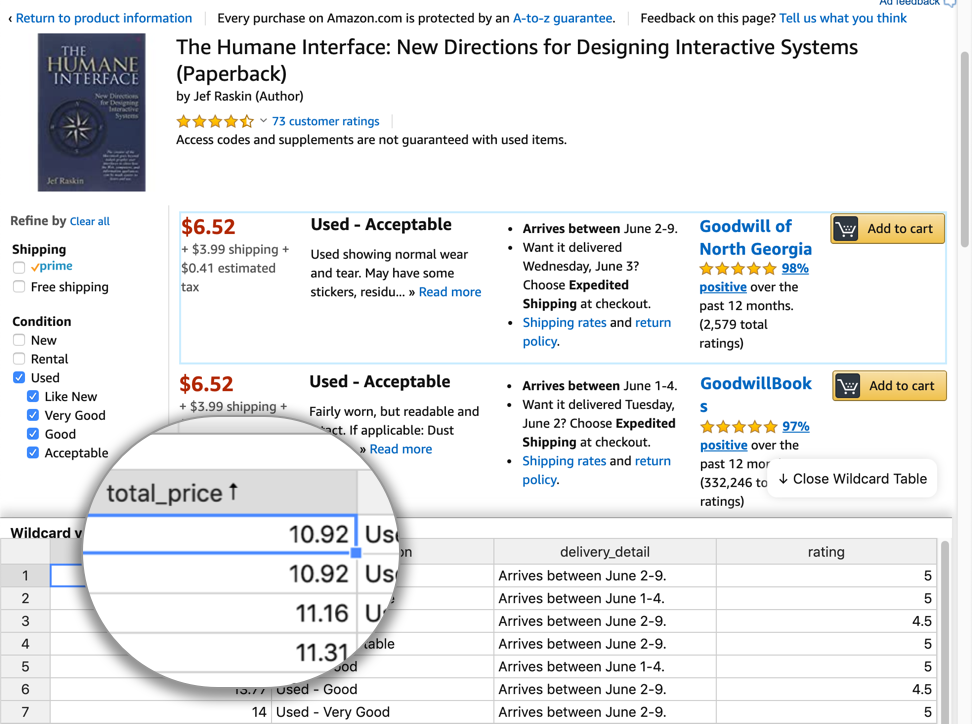
\includegraphics[width=\columnwidth]{media/amazon.png}
\caption{Sorting the used sellers page on Amazon by total price, including fees. The original page doesn't have sorting, and doesn't show the combined price.}\label{fig:amazon}
}
\end{figure}

\begin{figure}
\hypertarget{fig:ubereats}{%
\centering
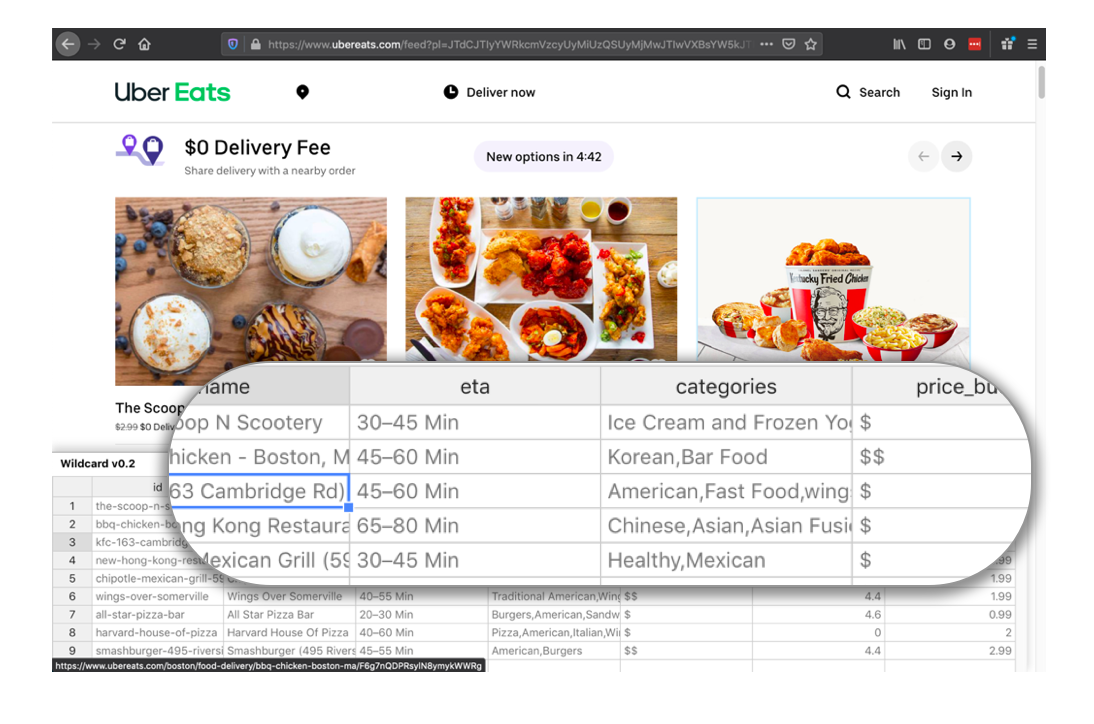
\includegraphics[width=\columnwidth]{media/ubereats.png}
\caption{Organizing takeout restaurants on Uber Eats by delivery ETA and price}\label{fig:ubereats}
}
\end{figure}

\hypertarget{annotating}{%
\subsubsection{Annotating}\label{annotating}}

Many web annotation systems focus on annotating text or arbitrary
webpage content, but Wildcard limits annotations to structured objects
extracted by an adapter, resulting in a different set of use cases.
Annotating with Wildcard has proven most useful when taking notes on a
list of possible options (e.g., evaluating possible Airbnb locations to
rent). We have also used it with Instacart's online grocery cart, for
jotting down notes as we review an order and consider modifications
(shown in Figure~\ref{fig:instacart}).

\hypertarget{formulas}{%
\subsubsection{Formulas}\label{formulas}}

Formulas are the most powerful part of the Wildcard system. So far, our
language supports only a small number of predefined functions. Adding
more should allow a broad range of useful computations, as shown by the
success of spreadsheets.

Formulas are especially useful for fetching data from Web APIs. We've
used them to augment Airbnb listings with walkability scores, and to
augment Hacker News articles with estimated read times as shown in
Section~\ref{sec:example}. One challenge of the current language design
is that supporting a new web API requires writing Javascript code to add
a new function to the language, because web APIs typically return
complex JSON data structures that can't be easily displayed in a single
table cell. In the future we would like to make it possible to call new
APIs without adding a dedicated function, which might require adding
functions to the formula language that can manipulate JSON data.

We have also found instances where simple data manipulation is useful,
e.g.~transforming the results of an API call with basic arithmetic and
string operations, as shown in Section~\ref{sec:example}.

\begin{figure}
\hypertarget{fig:instacart}{%
\centering
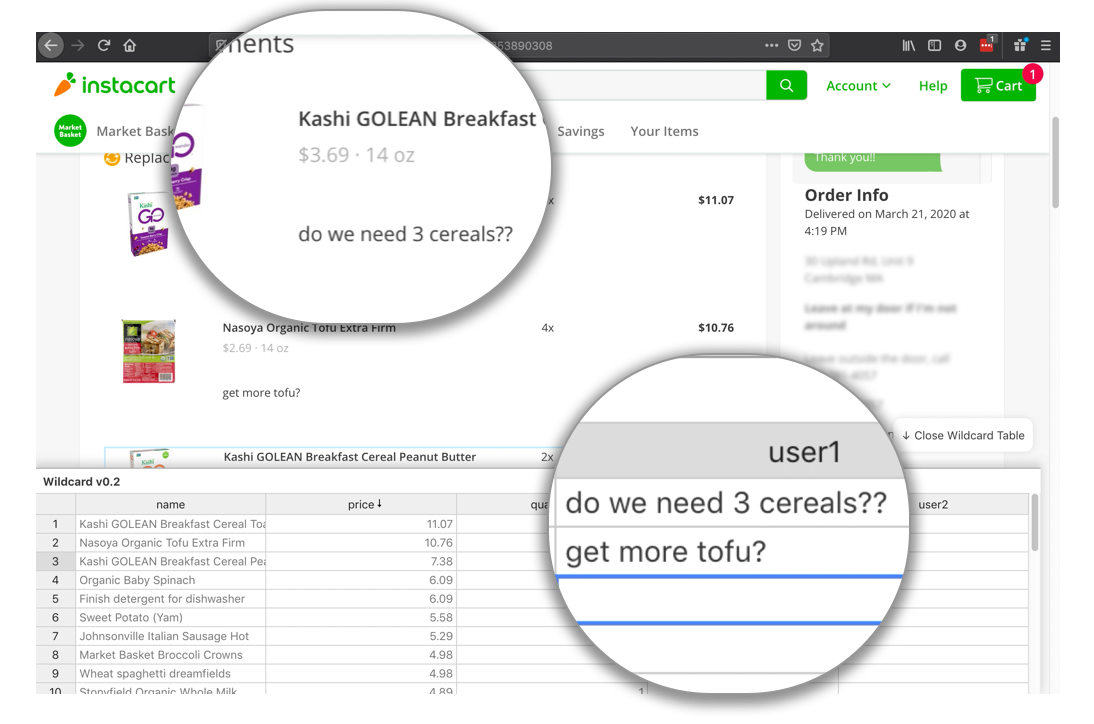
\includegraphics[width=\columnwidth]{media/instacart.png}
\caption{Taking notes on Instacart grocery items, after sorting them by price}\label{fig:instacart}
}
\end{figure}

\hypertarget{cell-editors}{%
\subsubsection{Cell editors}\label{cell-editors}}

We developed two cell editors, to explore the benefits of adding custom
UI for editing values in the table.

One valuable feature is that users can incorporate their private
information into a web UI. We created a datepicker based on the
\href{https://fullcalendar.io/}{FullCalendar} plugin, which can load
data from a Google Calendar. This makes it convenient to enter dates
into a website based on the user's personal calendar information,
without uploading that information to the website itself.

Another benefit is that a user can choose a preferred widget for editing
information across different sites that typically provide a fragmented
editing experience. We built a text editor based on the
\href{https://ckeditor.com/}{CKEditor} rich text editor, and integrated
it with Google's Blogger website by representing the contents of a blog
post as a single table cell containing an HTML string (shown in
Figure~\ref{fig:blogger}). If there were site adapters available for
other websites with rich text entry, the user could then use a single
rich text editor to edit text across the whole web.

\begin{figure}
\hypertarget{fig:blogger}{%
\centering
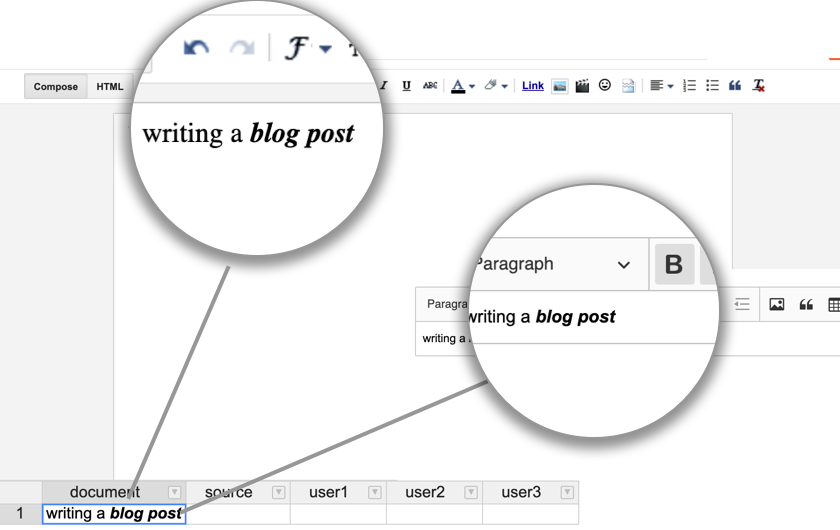
\includegraphics[width=\columnwidth]{media/blogger.png}
\caption{Using a custom text editor widget to edit a blog post on Blogger. The text is synchronized with the Blogger editor through a table cell.}\label{fig:blogger}
}
\end{figure}

\hypertarget{limitations}{%
\subsubsection{Limitations}\label{limitations}}

There are many customizations that are not possible to implement with
data-driven customization. Some of the limitations are specific to the
current implementation of the Wildcard extension, but others are more
fundamental to the general paradigm.

One limitation is that Wildcard can only make customizations that use
the available data exposed in the table. If the adapter doesn't expose
some piece of data, the user can't use it in their customization. The
table data format also rules out customizing certain sites that don't
have a way to map to a table. The UI modifications available in Wildcard
are also limited in scope; deleting arbitrary buttons isn't possible,
for example. There is no facility for running automations when the user
isn't actively viewing a page---at one point, we wanted to build an
automation to repeatedly load a grocery delivery website to check for
open delivery slots, but it didn't seem possible to achieve this in
Wildcard.

We consider these limitations to be an acceptable outcome. Our goal is
to support as many useful customizations as possible with a low
threshold of difficulty, and not to span all possible customizations. If
users want to implement more sophisticated customizations, they have the
option of graduating to more advanced customization tools like scripting
languages.

We have found that one benefit of showing structured data is
predictability: once we build an adapter for a website, it is clear what
data is available or unavailable for use in customizations. Also, there
is sometimes a way to reframe an imperative script in terms of our
direct manipulation model. For example, a script that iterates through
rows in a page adding some additional information to each row can be
reproduced using a single formula in Wildcard.

\hypertarget{viability-of-scraping}{%
\subsection{Viability of scraping}\label{viability-of-scraping}}

Our second evaluation area relates less to the conceptual approach of
data-driven customization, and more to the specific implementation of
customizing existing web applications. In order for third-party
customization through Wildcard to succeed, it is important that creating
usable adapters for existing websites takes minimal effort.

Nearly all of our DOM scraping adapters were created by members of our
team. However, an external developer unaffiliated with the project
contributed one adapter, designed to sort the Github page listing a
user's repositories, and they described the experience as ``very
straightforward.''

The adapters for our test sites ranged from 36 to 117 lines of code,
averaging 68 lines; Table 1 shows the number of lines of code for each
adapter. Most of the code in the adapters is simply using DOM APIs and
CSS selectors to implement conventional web scraping logic.

Some of the challenges of writing a DOM scraping adapter are the same
ones as with writing normal web scraping code. Sometimes, addressing the
desired set of elements can be difficult, and when sites change,
scrapers can break---we observed several instances where sites changed
their CSS classes and caused Wildcard adapters to no longer work. One
benefit of a library of shared wrappers is that if many customizations
depend on some piece of scraping logic, rather than having the scraping
logic embedded in a single browser extension, it should be more likely
to be fixed quickly.

The interactive nature of Wildcard also introduces additional challenges
beyond normal web scraping. One challenge is registering appropriate
event handlers to update the table data in response to UI changes that
happen after initial page load. Another challenge is persisting updates
to the DOM---some websites use virtual DOM frameworks that can
occasionally overwrite changes made by Wildcard. So far, in practice
we've managed to work around these issues for all of the websites we've
tried, but we don't claim that any website can be customized through DOM
scraping. As web frontend code gets increasingly complex (and starts to
move beyond the DOM to other technologies like Shadow DOM or even
WebGL), it may become increasingly difficult to customize websites from
the outside without first-party support.

AJAX scraping proved very useful in several cases. The Uber Eats website
was challenging to scrape because it has a complex DOM structure with
machine-generated CSS classes, but the site also uses AJAX requests
which contain all the relevant data in a structured form that is much
easier to extract. We also found examples where relevant information
wasn't present in the DOM at all. On the grocery delivery site
Instacart, we found that AJAX requests contained additional data not
shown in the UI, enabling us to do things like sort grocery items by
category.

\hypertarget{sec:visions}{%
\section{Vision}\label{sec:visions}}

\begin{itemize}
\tightlist
\item
  Wildcard just one instance of a broader data-driven customization

  \begin{itemize}
  \tightlist
  \item
    particular view: table
  \item
    particular context: web
  \end{itemize}
\item
  here we share some of the underlying ideas. go beyond Wildcard, room
  to grow
\end{itemize}

\hypertarget{sec:dm}{%
\subsection{Customization by direct manipulation}\label{sec:dm}}

Hutchins, Hollan and Norman \citep{hutchins1985} define a direct
manipulation interface as one that uses a model-world metaphor rather
than a conversation metaphor. Instead of presenting an ``assumed'' but
not directly visible world that the user converses with, ``the world is
explicitly represented'' and the user can ``{[}act{]} upon the objects
of the task domain themselves.''

Although most GUIs today employ direct manipulation, software
customization tools typically use an imperative programming model, which
implements the conversational metaphor rather than direct manipulation.
Here, for example, is how a user retrieves a list of of calendar names
from the Calendar application in Applescript \citep{cook2007}, the
scripting language for customizing Mac OS applications:

\begin{verbatim}
tell application "Calendar"
  name of calendars
end tell
\end{verbatim}

Some customization environments like Mac Automator and Zapier forego
textual syntax and let the user connect programs and construct
automations by dragging and dropping icons representing commands. These
environments still do not constitute direct manipulation, though: the
objects being manipulated are in the domain of programming, not in the
domain of the task at hand.

Imperative programming is a reasonable choice as the model for building
customizations. Turing-complete programming provides a high ceiling for
possible customizations, and a sequence of commands is a natural fit for
automations that simulate a series of steps taken by the user. There is,
however, a serious drawback to this approach. MacLean et
al.~\citep{maclean1990} describe an ideal for user-tailorable systems: a
``gentle slope'' from using to customizing, where small incremental
increases in skill lead to corresponding increments of customization
power. Requiring users wanting to customize their applications to learn
programming creates an abrupt ``cliff,'' exacting a significant
investment in learning even to implement the simplest customizations.
Another goal of MacLean et al.~is to make it ``as easy to change the
environment as it is to use it''---at least for some subset of changes.
But in scripting languages, the experience of customization does not
remotely resemble the experience of use.

With data-driven customization we aim to provide a gentler slope, by
using direct manipulation for software customization. The data shown in
the table view is the domain data from the original application. The
user makes changes to the data by selecting areas of interest in the
table, e.g.~sorting/filtering by clicking the relevant column header, or
adding annotations by clicking and typing on the relevant row. At every
step, the user receives intermediate feedback, not only in the table
view, but also in the original application, so it's clear whether they
are making progress towards their desired result. These types of
interactions are common in GUI applications, and Wildcard therefore
seems to meet MacLean et al.'s goal: some one-click customizations are
as easy as using the original application. Formulas introduce some
additional complexity, but spreadsheets have demonstrated that formula
programming is still accessible to many users, helped by the pure
functional semantics and the visibility of intermediate results.

One aspect of directness that we have chosen not to pursue in Wildcard
is enabling customization in closer proximity to the original user
interface elements, as explored by tools like Scotty
\citep{eagan2011}---all customization occurs in a separate panel next to
the original UI. While closer proximity might be helpful, we have found
that augmenting the original UI with a distinct, additional
representation provides a more consistent experience across all
applications, and clearly shows what structured data is available to
work with. We also emphasize the map ping between the representations by
highlighting content in the original page, similiar to the way that
browser developer tools highlight the currently selected element in the
DOM inspector in the original page.

Ainsworth et al.~provide a helpful taxonomy of the value of multiple
representations \citep{ainsworth1999}. In their terms, Wildcard plays a
\emph{complementary role} by supporting a \emph{different set of tasks}
from the original application, while displaying \emph{shared
information}. Wildcard may also help construct \emph{deeper
understanding by subtraction}---by stripping away details and only
showing the essential data in an interface, Wildcard encourages thinking
of an application in terms of its core information, rather than the
specific capabilities provided by the current user interface. In our
anecdotal experience, we've often found that looking at a site's data in
table format tends to spur new ideas for customizations which weren't
evident from looking at the original UI.

As noted in Section~\ref{sec:reflections}, there are many customizations
that can be achieved in scripting languages that cannot be implemented
in Wildcard. We consider this an acceptable tradeoff in exchange for a
gentler slope in customization, and we show in Section~\ref{sec:example}
and Section~\ref{sec:reflections} that our model can implement many
useful customizations.

\hypertarget{semantic-wrappers}{%
\subsection{Semantic wrappers}\label{semantic-wrappers}}

\emph{Ad hoc customization tools} enable customization without using
official extension APIs, enabling a broader range of customizations on
top of more applications. For example, web browser extensions have
demonstrated the utility of customizing websites through manipulating
the DOM, without websites needing to provide explicit extension APIs.
However, ad hoc customization comes with a cost: these tools typically
operate at a low level of abstraction, e.g.~manipulating user interface
elements, rather than in a meaningful domain model. This makes it harder
for end users to write scripts, and makes the resulting scripts more
brittle as the specifics of a user interface change.

\emph{Anticipated customization tools}, in contrast, use explicit
extension APIs provided by the application developer. Examples of this
include accessing a backend web API, or writing a customization in
Applescript for an application that exposes its domain model to the
scripting language. The main benefit of this style is that it allows the
extension author to work with meaningful concepts in the application
domain---``create a new calendar event'' rather than ``click the button
that contains the text `new event'.''---which makes customizations
easier to build and more robust. However, the plugin API limits the
types of customizations that can be built, and many applications don't
have any plugin API.

With Wildcard, we use a hybrid approach that aims to provide the best of
both worlds. Third-party programmers implement site-specific adapters
that are internally implemented as ad hoc customizations, but externally
provide a high-level interface to the application, abstracting away the
details of the user interface. These wrappers are added to a shared
repository, available to all users of the system. When an end user is
using a site that already has an adapter, they benefit from a semantic
customization experience that avoids low-level details.

One way to view this approach is as introducing a new abstraction
barrier into third-party extension. Typically, a third party
customization script combines two responsibilities: 1) mapping the
low-level details of a user interface to semantic constructs (e.g.,
using CSS selectors to find certain page elements), and 2) handling the
actual logic of the specific customization. Even though the mapping
logic is often more generic than the specific customization, the
intertwining of these two responsibilities in a single script makes it
very difficult to share the mapping logic across scripts.

With Wildcard we propose a decoupling of these two layers: a repository
of shared wrappers maintained by programmers, and a separate repository
of specific customizations built on top of these wrappers. This general
architecture has been successfully demonstrated by projects like
\href{https://github.com/KartikTalwar/gmail.js/}{Gmail.js}, an open
source project that wraps the Gmail web client in a convenient API for
browser extensions to build on.

The success of semantic wrappers depends on a key hypothesis: that a
single wrapper created by a programmer can be used for many different
purposes by end users. Although we've validated that a single generic
adapter can support many customizations, so far the people making the
adapters have largely been the same people building customizations on
top of them, so more work is needed to fully test this hypothesis.

A helpful future addition would be to allow end users to create wrappers
themselves, so that more people could contribute to the shared library.
There are many existing projects exploring end-user web scraping (such
as Helena \citep{chasins2018}) which might prove helpful; however,
because the needs of a Wildcard adapter are slightly more complex than a
traditional web scraper (as discussed in
Section~\ref{sec:architecture}), further work might be needed to enable
end-user wrapper creation.

The distribution mechanism for semantic wrappers is also important for
encouraging an ecosystem of shared wrappers. Currently, the distribution
mechanism is simply merging the code for all adapters into the main
Wildcard codebase. This is the simplest workable solution, but has its
downsides: contributing involves a fairly high barrier of creating a
pull request on Github, and using newly contributed wrappers requires
installing a new version of the extension. In the future we might
explore other mechanisms, like an online repository that the extension
pulls from dynamically. Security is also a consideration---DOM scraping
adapters can execute arbitrary Javascript code, which opens up the
possibility of malicious adapters being contributed. Currently we plan
to solve this challenge with centralized code review, but another
approach we are considering is using or inventing a more restricted
domain-specific language for specifying scraping logic.

\hypertarget{generic-data-interfaces}{%
\subsection{Generic data interfaces}\label{generic-data-interfaces}}

\begin{itemize}
\item
  what makes a UI good for customization?

  \begin{itemize}
  \tightlist
  \item
    generic: can show data from many apps
  \item
    neutral: doesn't prioritize a particular use case, leaves the
    imagination open
  \item
    good affordances for performing common actions
  \end{itemize}
\item
  could be others besides a table

  \begin{itemize}
  \tightlist
  \item
    tree?
  \item
    text box?
  \item
    compose these?
  \end{itemize}
\end{itemize}

\hypertarget{decouple-data-from-application-logic}{%
\subsection{Decouple data from application
logic}\label{decouple-data-from-application-logic}}

\begin{itemize}
\item
  thin client architecture of web has promoted a coupling of data + app

  \begin{itemize}
  \tightlist
  \item
    only way user can view the data is in the first-party tool
  \item
    APIs provide some flexibility in picking a client. but, APIs aren't
    meant for end user consumption. and, there are limits (eg, Twitter
    API restrictions)
  \item
    limited user agency over how they use their data
  \item
    compare to, say, opening a file locally
  \end{itemize}
\item
  Some people aiming towards ambitious rearchitectures in this
  space\ldots{}

  \begin{itemize}
  \tightlist
  \item
    cite local-first
  \item
    TBL Solid
  \end{itemize}
\item
  Data-driven customization: an iterative approach towards this vision;
  complementary to more radical rearchitecting.
\item
  Start with third party extraction
\item
  Integrate across apps
\item
  open the data in a different UI
\item
  Then move to first party data providing in the client (could drive
  wildcard from existing apis??)
\end{itemize}

\hypertarget{sec:related-work}{%
\section{Related Work}\label{sec:related-work}}

This paper extends work reported in a workshop paper by Litt and Jackson
\citep{litt2020} which presented an early version of the Wildcard
extension. We have substantially extended their work in this paper by
creating the table adapter abstraction, reimplementing the internals of
Wildcard around that abstraction, evaluating the system on many more
websites and use cases, and by characterizing the design of the system
in much more detail than in their workshop paper.

data-driven customization relates to two broad areas of related work.
Our problem statement is related to software customization tools, and
our solution approach is related to spreadsheets and other direct
manipulation interfaces.

\hypertarget{customization-tools}{%
\subsection{Customization tools}\label{customization-tools}}

data-driven customization is most closely related to other tools that
aim to empower end users to customize software without traditional
coding.

This lineage goes back at least to the Buttons system by MacLean et
al.~\citep{maclean1990}, where Xerox Lisp users could share buttons that
performed various ``tailoring'' actions on the system. The authors
proposed the ``gentle slope'' idea which has greatly influenced our
approach to data-driven customization (as discussed in
Section~\ref{sec:dm}). The authors also point out the importance of a
``tailoring culture'' where people with different skillsets collaborate
to produce useful customizations; in their system, Lisp programmers
create buttons that others can use, modify, and rearrange. This division
of labor corresponds to our idea of semantic wrappers, where end user
customization is supported by programmer-created building blocks.

More recently, web customization tools have aimed to enable end users to
modify web interfaces without programming. Sifter \citep{huynh2006}
enables end users to sort and filter lists of data obtained by web
scraping, much like Wildcard's sorting features. The main difference
between the systems is that data-driven customization has many other use
cases besides sorting and filtering. Also, Sifter involves end users in
a semi-automated data extraction process, rather than having programmers
create wrappers. This provides coverage of more websites, but at the
expense of complicating the end user experience. We could integrate end
user scraping techniques in Wildcard in the future, but we believe that
when possible it's valuable for end users to have a customization
experience decoupled from the challenge of web scraping the underlying
data. Sifter also implements scraping across multiple pages, a valuable
feature for sorting and filtering that isn't present in Wildcard.

Thresher \citep{hogue2005} helps end users create wrappers that map
website content to Semantic Web schemas like ``Movie'' or ``Director,''
and augments websites with new functionality by exploiting that schema
information. Wildcard shares the general idea of wrappers, but maps to a
generic table data type rather than more specific schemas, increasing
the range of supported data and allowing for a simpler mapping process.

There are many software customization tools that offer simplified forms
of programming for end users. Chickenfoot \citep{bolin2005} and
Coscripter \citep{leshed2008} offer user friendly syntax for writing web
automation scripts; Applescript \citep{cook2007} has a similar goal for
desktop customization. There are visual programming environments for
customization that don't involve writing any text:
\href{https://support.apple.com/guide/automator/welcome/mac}{Automator}
for Mac and
\href{https://apps.apple.com/us/app/shortcuts/id915249334}{Shortcuts}
for iOS are modern options for customizing Apple products, and
\href{https://zapier.com/}{Zapier} enables users to connect different
web applications together visually. As mentioned previously, these tools
all require writing imperative programs, in contrast to the more
declarative and direct approach of data-driven customization.

\hypertarget{spreadsheets-and-visual-query-interfaces}{%
\subsection{Spreadsheets and visual query
interfaces}\label{spreadsheets-and-visual-query-interfaces}}

Another relevant area involves spreadsheets and visual query interfaces.
We take inspiration from these tools in our work, but apply them in a
different domain: customizing existing software applications, rather
than interacting with databases or constructing software from scratch.

The most closely related work is in systems that offer spreadsheet-like
querying of relational data. SIEUFERD by Bakke and Karger
\citep{bakke2016} is one such recent system, and their paper presents a
survey of many other similar tools. Our work is particularly influenced
by the authors' observation that a user should be able to modify queries
by interacting with the results of the query rather than some
representation of the query itself. SIEUFERD's interface supports a far
more general range of queries than Wildcard, but the core principles of
the user interface are the same. \href{https://airtable.com/}{Airtable}
is another example of a modern commercial product that offers
spreadsheet-like interaction with a relational database.

Our work is also inspired by the many projects that have explored using
spreadsheets as a foundation for building software applications,
including Object Spreadsheets \citep{mccutchen2016}, Quilt
\citep{benson2014}, Gneiss \citep{chang2014}, Marmite \citep{wong2007},
and \href{https://www.glideapps.com/}{Glide}. We share the main idea of
connecting a spreadsheet view to a GUI, but we apply it to software
customization, rather than building software from scratch.

Another related system is ScrAPIr, by Alrashed et
al.~\citep{alrashed2020}, which enables end users to access backend web
APIs without programming. ScrAPIr shares our high level goal of end user
empowerment, as well as the idea of wrappers, by creating a shared
library of wrappers around existing web APIs. Unlike Wildcard, however,
ScrAPIr targets explicit APIs exposed by developers. It also focuses on
backend services and doesn't aim to extend the frontend interfaces of
web applications.

\hypertarget{sec:conclusion}{%
\section{Conclusion and Future Work}\label{sec:conclusion}}

In this paper, we have presented data-driven customization, a new
paradigm for customizing software by direct manipulation of the
underlying structured data. We have demonstrated the paradigm using the
Wildcard browser extension, and have used it to create useful
customizations for a variety of websites.

So far, most usage of Wildcard has come from members of the project
team. Our primary goal for future work is to evaluate the system with a
broader group of users. What usability barriers do end users face when
using the system? What types of customizations do they choose to create?
What formulas prove most helpful? Through real deployment of the tool,
we hope to validate the viability of a community-maintained library of
site-specific adapters.

Another area for future work is exploring whether it's possible to
express a broader range of customizations by extending the table-editing
paradigm. Are there ways to offer an increase in power and functional
complexity, while retaining a programming model that is simpler for end
users than conventional coding? For example, one possibility would be to
enable users to set up triggers to perform actions like sending
notifications when certain conditions are met in the table view.

As computing plays an ever greater role in our lives, it is increasingly
important that end users have agency over the behavior of their
software, rather than having every detail be dictated by companies whose
incentives are not always aligned with the user's interests. We hope
that data-driven customization can serve as a point on the path from
normal use to deep modification, in support of a more adaptable
experience for all computer users.

%%
%% The next two lines define the bibliography style to be used, and
%% the bibliography file.
\bibliographystyle{ACM-Reference-Format}
\bibliography{wildcard-onward-bibtex.bib}

\end{document}
\endinput
%%
%% End of file `sample-sigconf.tex'.
